% GNUPLOT: LaTeX picture with Postscript
\begingroup
  \makeatletter
  \providecommand\color[2][]{%
    \GenericError{(gnuplot) \space\space\space\@spaces}{%
      Package color not loaded in conjunction with
      terminal option `colourtext'%
    }{See the gnuplot documentation for explanation.%
    }{Either use 'blacktext' in gnuplot or load the package
      color.sty in LaTeX.}%
    \renewcommand\color[2][]{}%
  }%
  \providecommand\includegraphics[2][]{%
    \GenericError{(gnuplot) \space\space\space\@spaces}{%
      Package graphicx or graphics not loaded%
    }{See the gnuplot documentation for explanation.%
    }{The gnuplot epslatex terminal needs graphicx.sty or graphics.sty.}%
    \renewcommand\includegraphics[2][]{}%
  }%
  \providecommand\rotatebox[2]{#2}%
  \@ifundefined{ifGPcolor}{%
    \newif\ifGPcolor
    \GPcolortrue
  }{}%
  \@ifundefined{ifGPblacktext}{%
    \newif\ifGPblacktext
    \GPblacktextfalse
  }{}%
  % define a \g@addto@macro without @ in the name:
  \let\gplgaddtomacro\g@addto@macro
  % define empty templates for all commands taking text:
  \gdef\gplbacktext{}%
  \gdef\gplfronttext{}%
  \makeatother
  \ifGPblacktext
    % no textcolor at all
    \def\colorrgb#1{}%
    \def\colorgray#1{}%
  \else
    % gray or color?
    \ifGPcolor
      \def\colorrgb#1{\color[rgb]{#1}}%
      \def\colorgray#1{\color[gray]{#1}}%
      \expandafter\def\csname LTw\endcsname{\color{white}}%
      \expandafter\def\csname LTb\endcsname{\color{black}}%
      \expandafter\def\csname LTa\endcsname{\color{black}}%
      \expandafter\def\csname LT0\endcsname{\color[rgb]{1,0,0}}%
      \expandafter\def\csname LT1\endcsname{\color[rgb]{0,1,0}}%
      \expandafter\def\csname LT2\endcsname{\color[rgb]{0,0,1}}%
      \expandafter\def\csname LT3\endcsname{\color[rgb]{1,0,1}}%
      \expandafter\def\csname LT4\endcsname{\color[rgb]{0,1,1}}%
      \expandafter\def\csname LT5\endcsname{\color[rgb]{1,1,0}}%
      \expandafter\def\csname LT6\endcsname{\color[rgb]{0,0,0}}%
      \expandafter\def\csname LT7\endcsname{\color[rgb]{1,0.3,0}}%
      \expandafter\def\csname LT8\endcsname{\color[rgb]{0.5,0.5,0.5}}%
    \else
      % gray
      \def\colorrgb#1{\color{black}}%
      \def\colorgray#1{\color[gray]{#1}}%
      \expandafter\def\csname LTw\endcsname{\color{white}}%
      \expandafter\def\csname LTb\endcsname{\color{black}}%
      \expandafter\def\csname LTa\endcsname{\color{black}}%
      \expandafter\def\csname LT0\endcsname{\color{black}}%
      \expandafter\def\csname LT1\endcsname{\color{black}}%
      \expandafter\def\csname LT2\endcsname{\color{black}}%
      \expandafter\def\csname LT3\endcsname{\color{black}}%
      \expandafter\def\csname LT4\endcsname{\color{black}}%
      \expandafter\def\csname LT5\endcsname{\color{black}}%
      \expandafter\def\csname LT6\endcsname{\color{black}}%
      \expandafter\def\csname LT7\endcsname{\color{black}}%
      \expandafter\def\csname LT8\endcsname{\color{black}}%
    \fi
  \fi
  \setlength{\unitlength}{0.0500bp}%
  \begin{picture}(7936.00,2834.00)%
    \gplgaddtomacro\gplbacktext{%
      \csname LTb\endcsname%
      \put(-63,879){\makebox(0,0)[r]{\strut{}\scriptsize -0.3}}%
      \put(-63,1124){\makebox(0,0)[r]{\strut{}\scriptsize -0.2}}%
      \put(-63,1369){\makebox(0,0)[r]{\strut{}\scriptsize -0.1}}%
      \put(-63,1615){\makebox(0,0)[r]{\strut{}\scriptsize 0}}%
      \put(-63,1860){\makebox(0,0)[r]{\strut{}\scriptsize 0.1}}%
      \put(-63,2105){\makebox(0,0)[r]{\strut{}\scriptsize 0.2}}%
      \put(-63,2350){\makebox(0,0)[r]{\strut{}\scriptsize 0.3}}%
      \put(218,377){\makebox(0,0){\strut{}\scriptsize -0.4}}%
      \put(764,377){\makebox(0,0){\strut{}\scriptsize -0.2}}%
      \put(1309,377){\makebox(0,0){\strut{}\scriptsize 0}}%
      \put(1854,377){\makebox(0,0){\strut{}\scriptsize 0.2}}%
      \put(2400,377){\makebox(0,0){\strut{}\scriptsize 0.4}}%
      \put(-569,1614){\rotatebox{-270}{\makebox(0,0){\strut{}$u_{R}$ (\AA)}}}%
      \put(1309,91){\makebox(0,0){\strut{}}}%
      \put(794,2720){\makebox(0,0)[l]{\strut{}\scriptsize{$\lambda_{ir} = 0.00$ eV}}}%
    }%
    \gplgaddtomacro\gplfronttext{%
    }%
    \gplgaddtomacro\gplbacktext{%
      \csname LTb\endcsname%
      \put(2836,377){\makebox(0,0){\strut{}\scriptsize -0.4}}%
      \put(3382,377){\makebox(0,0){\strut{}\scriptsize -0.2}}%
      \put(3928,377){\makebox(0,0){\strut{}\scriptsize 0}}%
      \put(4473,377){\makebox(0,0){\strut{}\scriptsize 0.2}}%
      \put(5019,377){\makebox(0,0){\strut{}\scriptsize 0.4}}%
      \put(3278,1614){\rotatebox{-270}{\makebox(0,0){\strut{}}}}%
      \put(3927,47){\makebox(0,0){\strut{}$u_{ir}$ (\AA)}}%
      \put(3412,2720){\makebox(0,0)[l]{\strut{}\scriptsize{$\lambda_{ir} = 0.1263$ eV}}}%
    }%
    \gplgaddtomacro\gplfronttext{%
    }%
    \gplgaddtomacro\gplbacktext{%
      \csname LTb\endcsname%
      \put(5455,377){\makebox(0,0){\strut{}\scriptsize -0.4}}%
      \put(6001,377){\makebox(0,0){\strut{}\scriptsize -0.2}}%
      \put(6546,377){\makebox(0,0){\strut{}\scriptsize 0}}%
      \put(7091,377){\makebox(0,0){\strut{}\scriptsize 0.2}}%
      \put(7637,377){\makebox(0,0){\strut{}\scriptsize 0.4}}%
      \put(5897,1614){\rotatebox{-270}{\makebox(0,0){\strut{}}}}%
      \put(6546,91){\makebox(0,0){\strut{}}}%
      \put(6031,2720){\makebox(0,0)[l]{\strut{}\scriptsize{$\lambda_{ir} = 0.25$ eV}}}%
    }%
    \gplgaddtomacro\gplfronttext{%
    }%
    \gplbacktext
    \put(0,0){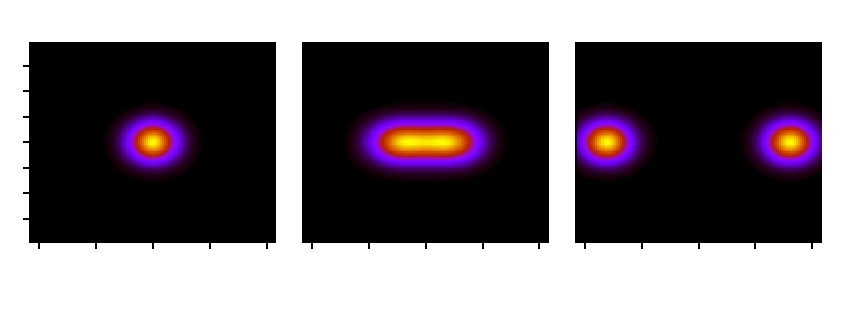
\includegraphics{images/phononProjGrd}}%
    \gplfronttext
  \end{picture}%
\endgroup
